\newpage
\chapter{Analýza}
\label{ch:Analýza}
V tejto časti sa venujeme dôkladnej analýze podkladov. Jednotlivé časti sú popísané v rozsahu relevantnom pre túto prácu. Analýza je štrukturovaná na nasledovné časti:

\begin{my_itemize}
	\item {Problémová oblasť}
	\item {Dáta sprístupnené pre prácu}
	\item {Neurónové siete}
	\item {Výskum v danej oblasti}
\end{my_itemize}

\section{Problémová oblasť}
\label{analyza_problemova_oblast}

V tejto práci sa zameriavame na predikciu úbytku zákazníkov(churn rate) pri predplatiteľských službách. V súčasnej dobe sa do popredia biznis prístupov stále viac dostávajú prístupy riadenia vzťahov zo zákazníkmi(CRM). Ukazuje sa totiž, že na trhu s dostatočným pokrytím poskytovateľov cieľovej služby je niekoľkonásobne drahšie získať nového ako udržať si existujúceho zákazníka. Tento prístup však vyžaduje rozsiahlu znalosť dostupnej zákazníckej základne, ktorou poskytovateľ disponuje. \newline

\subsection{Predikcia úbytku zákazníkov}
\label{analyza_ubytok_zakaznikov}

Predikcia úbytku zákazníkov sa venuje spracovaniu dostupných dát o zákazníckej aktivite, službách ktoré využívajú a vývoja ich správania v čase. Výsledkom analýzy je štatistika poskytujúca informácie o jednotlivých zákazníkoch a ich šanci na presun k inému poskytovateľovi. Z týchto dát je následne odvoditeľné, aké percento zákazníkov odíde ku konkurencii a aký to bude mať dopad na finančné príjmy od ktorých je poskytovateľ závislý. 

\subsection{Moderovanie úbytku zákazníkov}
\label{analyza_moderovanie_ubytku}

Vo vzťahu k úbytku zákazníkov definuje CRM dva základné prístupy, ktorými je možné moderovať úbytok. 

\subsubsection{Reaktívny prístup}
\label{analyza_reaktivny_pristup}

Motivácia zákazníka pre zotrvanie s pôvodným poskytovateľom služby nastáva, až keď sa zákazník explicitne rozhodne pre prechod ku konkurenčnému poskytovateľovi. V tomto okamihu začína poskytovateľ na svojho zákazníka apelovať výhodnými ponukami, zľavami alebo inými spôsobmi motivácie pre zotrvanie u poskytovateľa. Takýto prístup sa ukazuje ako ľahko zneužiteľný ostatnými zákazníkmi, ktorí by inak nemali motiváciu pre prechod ku konkurencii. Predikcia úbytku zákazníkov v tomto prístupe nemá nijakú významnú úlohu.

\subsubsection{Proaktívny prístup}
\label{analyza_proaktivny_pristup}

Pri úspešnej predikcii záujmu zákazníka o prechod ku konkurenčnému poskytovateľovi je možné efektívne jeho zámer smerovať pozitívnou motiváciou. Tento prístup však predpokladá vysokú úspešnosť predikčných metód. Pri nesprávnej identifikácii zákazníckeho správania je totiž nielen možné nezabrániť zákazníkom v presune ku konkurenčnému modelu, ale aj investícii finančných prostriedkov do skupiny zákazníkov, ktorá by naďalej generovala zisk aj bez významnejšej motivácie, resp. nevrátila by rozdielom v úbytku motivačné náklady, ktoré na ňu daný poskytovateľ vynaložil.

\section{Dáta sprístupnené pre prácu}
\label{analyza_data}

Pre túto prácu boli sprístupnené dáta z platobnej brány portálu pre online spravodajské denníky. Platobný portál poskytuje platformu pre periodiká, ktoré majú záujem o online funkcionalitu ale nemajú záujem implementovať vlastný platobný systém. Zákazníci tohto portálu tak získavajú rýchle riešenie pre možnosť vyhradenia exkluzívneho obsahu zo svojich online materiálov.

\subsection{Exkluzívny obsah}
\label{analyza_exkluzivny_obsah}

Exkluzívny obsah je nástroj, ktorý množstvo poskytovateľov služieb využíva pri prechode na web. Umožňuje prístup k väčšiemu počtu potenciálnych zákazníkov, pričom poskytovateľovi ostáva možnosť oddeliť, čo bude prístupné každému od exkluzívneho obsahu určeného pre predplatiteľov. \newline
Realizáciu exkluzívneho obsahu pomocou platobnej brány tretej strany umožňuje špecifikácia VAW(value added web). VAW aplikuje TINA(Telecommunications Information Networking Architecture) biznis model do klasického WWW(world wide web) prostredia.  Určuje tak vzťahy medzi jednotlivými právnymi subjektami podľa obr.~\ref{fig:vaw}. Poskytovateľ služieb(spravodajské periodikum) tak môže poskytovať nielen klasický ale aj exkluzívny obsah bez toho, aby sa vo väčšej miere muselo zaoberať správou poskytovaných služieb a finančnou administratívou. Za tú zodpovedá sprostredkovateľ(platobný portál), ktorého úloha spočíva v správe exkluzívneho obsahu vo vzťahu ku koncovému používateľovi.

\begin{figure}[H]
\begin{center}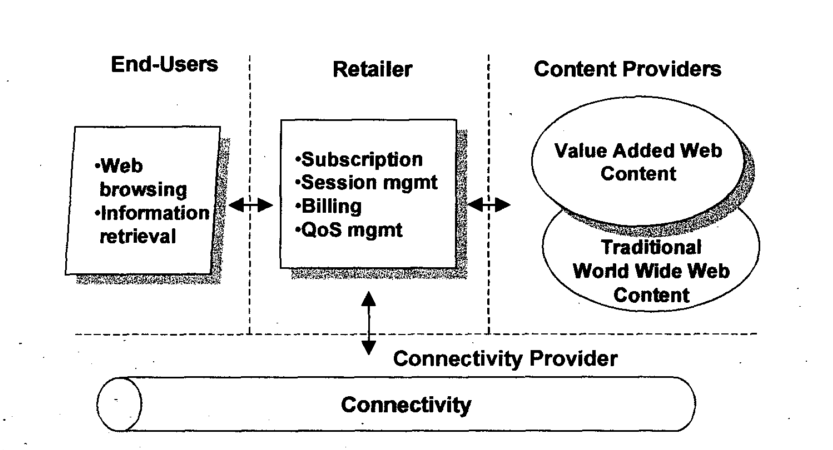
\includegraphics[scale=0.48]{vaw}\end{center}
\caption[vaw]{Základná schéma VAW}\label{fig:vaw}
\end{figure}

\subsection{Získavanie dát}
\label{analyza_ziskavanie_dat}

Pri pokuse o prístup k exkluzívnemu obsahu stojí medzi používateľom a obsahom platobná brána portálu. Používateľovi bez predplatenej služby je zobrazená ponuka na platený prístup. Predplatitel prechádza cez bránu a je mu sprístupnený exkluzívny obsah. Pri všetkých aktivitách na portáli sú zaznamenávané používateľské údaje. Dostupné údaje sú vo forme záznamov - textových súborov priebežne generovaných používateľskou činnosťou. 
Bežná činnosť pri analýze záznamov z činnosti a práci s velkými dátami všeobecne je predspracovanie dát. Pri sledovaní činnosti používateľov sa generujú súbory so stovkami miliónov až miliardami záznamov. V súčasnosti nie je možné klasickými prístupmi spracovať takéto objemy dát bez predspracovania - filtrovania, segmentácie a čistenia dát. Spôsob predspracovania dát je z podstatnej časti ovplyvnený metódami, ktorými chceme dáta spracovať. Pri práci so záznamami je bežné deliť dáta na tzv. používateľské prístupy (user sessions). Používateľský prístup modeluje aktivitu - jeden prístup jedného používateľa. Všeobecne platí, že ak používateľ dosiahne v činnosti pauzu 30 a viac minút, jedná sa o samostatný nový prístup. Takto rozdelené záznamy poskytujú elasticitu pri spracovaní podľa špecifického času alebo podľa používatelov. 

Medzi najdôležitejšie dostupné údaje z platobného portálu patria:

\begin{my_itemize}
	\item {IP adresa}
	\item {Používateľský účet}
	\item {Časový rozsah prístupu}
	\item {Prehliadaný obsah}
	\item {Aktivácia/prerušenie predplatného}
\end{my_itemize}

\section{Neurónové siete}
\label{analyza_neuronove_siete}
%citovat deeplearning.org

Koncept neurónových sietí vznikol v 40. rokoch minulého storočia inšpiráciou biologickými neurónovými sieťami v mozgu. Cieľom bolo prekonať bariéru medzi tým, čo je pre ľudský mozog ľahko riešitelné ale ťažko formálne definovatelné matematickými pravidlami. Tieto problémy, ktoré riešime intuitívne, pri pokuse o formálnu špecifikáciu ukazujú, aké množstvo znalostí používame v každodennom živote. Ako vhodný príklad slúži vizuálne rozoznávanie objektov, ktoré je pre osobu samozrejmé, no až v posledných rokoch zaznamenávame prvé úspechy v tejto problematike pri použití NN.  

\subsection{Štruktúra}
\label{analyza_struktura_nn}

Podobne ako v mozgu, základ neurónovej siete tvoria neuróny a prepojenia medzi nimi. Neuróny sú organizované vo vrstvách, ktoré sa delia na 3 základné typy. 
%\newline
\noindent

\textbf{Vstupná vrstva} - reprezentuje dáta, ktoré podsúvame sieti pre interpretáciu. Dáta musia byť pred posunutím vstupnej vrstve často predspracované, aby bola sieť schopná interpretovať ich. Počet neurónov na vstupnej vrstve je ovplyvnený množstvom dát, ktoré máme na vstupe. V sieti existuje iba jediná vstupná vrstva.
%\newline
\noindent

\textbf{Výstupná vrstva} - interpretácia dát sieťou. Výstupnú vrstvu je možné nazvať ,,výsledok"  siete.
\noindent

\textbf{Skrytá vrstva} - nachádzajú sa medzi vstupnou a výstupnou vrstvou. Ich počet určuje hĺbku siete. NN nemusí mať ani jednu skrytú vrstvu, no takáto sieť dokáže modelovať iba lineárnu závislosť. Všeobecne platí, že čím viac skrytých vrstiev má sieť, tým zložitejšie vzťahy dokáže simulovať. Zvyšujú sa však aj nároky na učenie a výpočtové nároky. Jediná skrytá vrstva vytvára pozoruhodný rozdiel v aplikovatelnosti modelu, keďže prekonáva hranicu lineárnej závislosti funkcie, ktorú model pokrýva. Pri vysokej zložitosti modelu je možné naraziť na problém preučenia, ktorý bráni sieti korektne generalizovať. Neexistuje nijaký spoľahlivá metóda pre správny počet alebo veľkosť skrytých vrstiev. Empiricky sa vyvinulo niekoľko odhadov, ale v praxi je nutné overovať správnosť modelu praktickou evaluáciou. Odhadové pravidlá najčastejšie padajú na neschopnosti integrovať vo svojom rozhodnutí komplexitu úlohy a redundanciu v tréningových dátach.
%\newline
\noindent

\textbf{Prepojenia} - Váhované prepojenia medzi neurónmi fungujú ako pamäť neurónovej siete. V jednoduchom modeli neurónovej siete sú prepojenia iba medzi neurónmi navzájom susediacich vrstiev. Prepojenie existuje medzi každým neurónom \textit{n}-tej do \textit{n+1} vrstvy. Neuróny jednej vrstvy pritom medzi sebou nie sú prepojené. Signál sa šíri týmito prepojeniami od vstupnej vrstvy smerom k výstupnej vrstve v jednom smere, ako je to ilustrované na obr.~\ref{fig:fnn}. Takéto siete sa volajú \textit{dopredné}. Hlavný účel prepojenia je niesť váhu. Váha prepojenia určuje, aký významný je vzťah medzi dvomi danými neurónmi, ktoré spája. Korektná váha daného prepojenia je na začiatku neznáma, jej korektné nastavenie je výsledkom procesu učenia.
%\newline
\noindent

\textbf{Neurón} - predstavuje základnú stavebnú jednotku neurónovej siete. Skladá sa z \textit{aktivačnej funkcie} a \textit{prahovej hodnoty}. Prahová hodnota neurónu $\vartheta _{i}^{k+1}$  je odpočítaná od sumy vstupných váhovaných hodnôt $ w_{ij}^{k}\, .\, o_{j}^{k}$. 
\newline
Na výsledok $o_{i}^{k+1}$ sa následne aplikuje aktivačná funkcia $f$ podľa obr.~\ref{fig:neuronoutput}. Takýto výstup je následne prepojeniami posielaný do ďaľších neurónov. Špeciálny prípad je neurón vstupnej a výstupnej vrstvy. Na vstupe totiž neurón hodnotu iba posiela ďalej a na výstupe po spracovaní nie je zasielaná nikam - predstavuje výsledok siete.
\newline



%\[o_{i}^{k+1}= f\left ( \sum_{j=1}^{N} w_{ij}^{k}\, .\, o_{j}^{k}\, -\, \vartheta _{i}^{k+1} \right )\]

%citovat kvasnicku a pospichala
\begin{figure}[H]
\begin{center}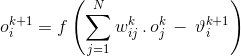
\includegraphics[scale=0.64]{neuronoutput}\end{center}
\caption[neuronoutput]{Výstupná hodnota neurónu}\label{fig:neuronoutput}
\end{figure}

%\newline
\noindent


%citovat a tutorial on training reccurent NN z mendeleya
\begin{figure}[H]
\begin{center}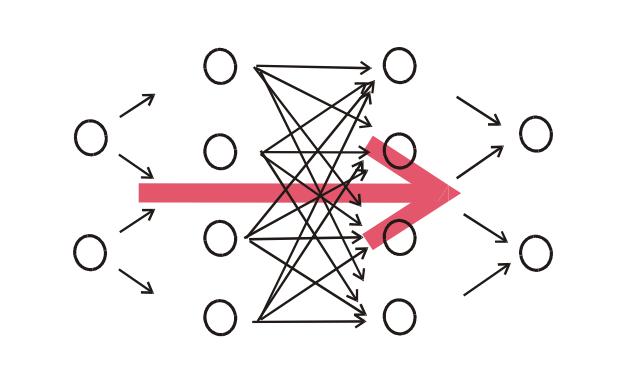
\includegraphics[scale=0.64]{fnn}\end{center}
\caption[fnn]{Štruktúra doprednej neurónovej siete (FNN)}\label{fig:fnn}
\end{figure}

\subsection{Učenie neurónovej siete}
\label{analyza_ucenie_nn}

Učenie predstavuje kľúčovú aktivitou pre schopnosť siete produkovať požadované výsledky. Spočíva vo vystavovaní neurónovej siete tréningovým dátam, ktoré sa sieť snaží interpretovať.

 %semi-supervidsed learning, active learning, reinforced learning
\textbf{Učenie s učiteľom} je metóda, pri ktorej je dostupná sada tréningových dát ,,označená". Pri interpretovaní výsledku je možné okamžite určiť, aká chyba nastala a následne ju propagovať do siete. Na toto sa využíva tzv. \textit{spätná propagácia}(backpropagation), ktorá upravuje váhy siete v rozsahu chyby, ktorá nastala - rozdiel medzi správnym výsledkom pre daný vstup a samotným výsledkom siete.
\noindent

\textbf{Učenie bez učiteľa} predstavuje alternatívnu metódu, pri ktorej tréningové dáta nemajú dostupné výsledky. Neurónová sieť sa sama učí rozhodnúť, čo je pre ňu relevantné. Učenie bez učiteľa predstavuje možnosť ako získať takmer neobmedzené množstvá tréningových dát tam, kde učenie s učiteľom vyžaduje manuálne a kvôli časovej náročnosti nedostupné označovanie.
\noindent

%deeplearning.org
\subsection{Hyperparametre}
\label{analyza_hyperparametre}

Nastavenia, pomocou ktorých kontrolujeme správanie neurónových sietí sa nazývajú \textit{hyperparametre}. Tieto hodnoty nie sú získané učením siete pokiaľ nemodelujeme vnorený systém za týmto účelom. Príkladom hyperparametra je počet skrytých vrstiev NN. Pri nízkom počte nebude model schopný naučiť sa funkciu definovanú problémom. Pri vysokom počte je možné, že sieť v sebe uloží menší tréningový dataset, nazývané tiež ako problém \textit{preučenia}(overfitting). Pri preučení sieť nezíska schopnosť generalizácie problému kvôli sledovaniu tréningového datasetu. Je zjavné, že zvolenie správnych hyperparametrov má pre výsledky metódy kľúčovú úlohu. Medzi ďaľšie významné hyperparametre patria:
\begin{my_itemize}
	\item {Šírka jednotlivých vrstiev}
	\item {Rýchlosť učenia}
	\item {Momentum}
	\item {Aktivačné funkcie neurónov}
\end{my_itemize}


%citovat a tutorial on training reccurent NN z mendeleya a deeplearning org
\subsection{Rekurentné neurónové siete}
\label{analyza_pokrocile_modely_nn}

Do popredia výskumu sa v súčasnosti dostávajú pokročilé modely, ktoré už nie sú obmedzené na jednoduchý dopredný prístup. Vďaka rapídnemu zvyšovaniu výkonu grafických kariet sa čoraz častejšie aplikujú \textit{rekurentné modely neurónových sietí}(RNN). Špecializáciou rekurentných sietí je práca so sekvenčnými dátami. Tieto siete predstavujú generalizáciu dopredných modelov ich rozšírením o cyklické prepojenia. Takýmto spôsobom je možné využiť súčasnú hodnotu premennej na ovplyvnenie vlastnej hodnoty v budúcnosti. Cyklický charakter rekurentného modelu je zobrazený na obr.~\ref{fig:rnn}.

%citovat a tutorial on training reccurent NN z mendeleya
\begin{figure}[H]
\begin{center}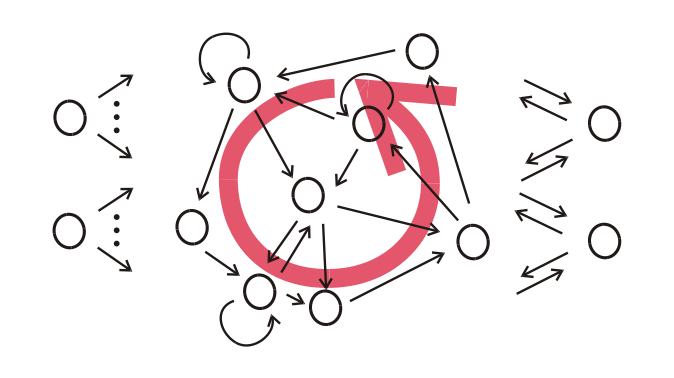
\includegraphics[scale=0.64]{rnn}\end{center}
\caption[rnn]{Štruktúra rekurentnej neurónovej siete}\label{fig:rnn}
\end{figure}

\subsection{Siete s dlhou krátkodobou pamäťou - LSTM}

%perfektne zdroje k LSTM aj odkazy v deeplearning.org pdf
LSTM predstavuje vylepšený model RNN. Vnútorná štruktúra ako doplnok ku externej rekurencii medzi jednotlivými neurónmi obsahuje aj \textit{internú rekurenciu}, zobrazenú v štruktúre LSTM neurónu na obr.~\ref{fig:lstm}. Medzi najdôležitejšie súčasti tohto modelu patria sigmoidné brány, ktoré rozhodujú o tom, ako sa signál bude širiť. LSTM tak prekonáva problém strácajúceho sa gradientu, ktorým trpí klasická RNN architektúra.
\newline
\textbf{Brána zabudnutia} ovplyvňuje, či nastáva vnútorná rekurencia neurónu. Stav tak môže ale nemusí byť faktorom ovplyvňujúcim nasledujúcu iteráciu výpočtu v sieti. Významné zlepšenie v LSTM sieťach prišlo s myšlienkou \textit{kontextom podmieneného zabúdania}. Takýto model sa ukazuje extrémne výhodným pri riešení problémov zahŕňajúcich \textit{časové pauzy}(lags).
%citovat "Learning precise timing with LSTM"
 Dôležitý prvok  na obr.~\ref{fig:lstm} predstavuje čierna kocka. Označuje pauzu o veľkosti jednej iterácie. Hodnota signálu tak ovplyvňuje nasledujúcu iteráciu, tj. vplýva na neskoršie udalosti.
\newline
\noindent
%citovat "Learning precise timing with LSTM"
%ako do riti mam prelozit peepholes? 
\textbf{Nazeracie diery}(peepholes) predstavujú vylepšenie LSTM. Rieši problémy, ktoré vznikajú na základe faktu, že brána nedostáva priame informácie o stave jadra LSTM bloku(CEC). Táto situácia nastáva, keď je výstupná brána zatvorená. \textit{Nazeranie} predstavuje techniku váhovaného prepojenia CEC s bránami bloku daného jadra. Prepojenia sú štandardné s výnimkou časovej pauzy. Schéma nazerania v LSTM bloku je zobrazená na obr.~\ref{fig:peepholes}.

LSTM siete v praxi dokázali svoje schopnosti pri aplikácií na rôzne netriviálne dátové problémy. Pozornosť je kladená na frekventovanú časovú závislosť v dátach:
%deeplearning LSTM ma odkazy na konkretne projekty
\begin{my_itemize}
	\item{Rozoznávanie rukopisu}
	\item{Generovanie rukopisu}
	\item{Rozoznávanie reči}
	\item{Označovanie obrázkov}
\end{my_itemize}

%citovat "Learning precise timing with LSTM"
\begin{figure}[H]
\begin{center}
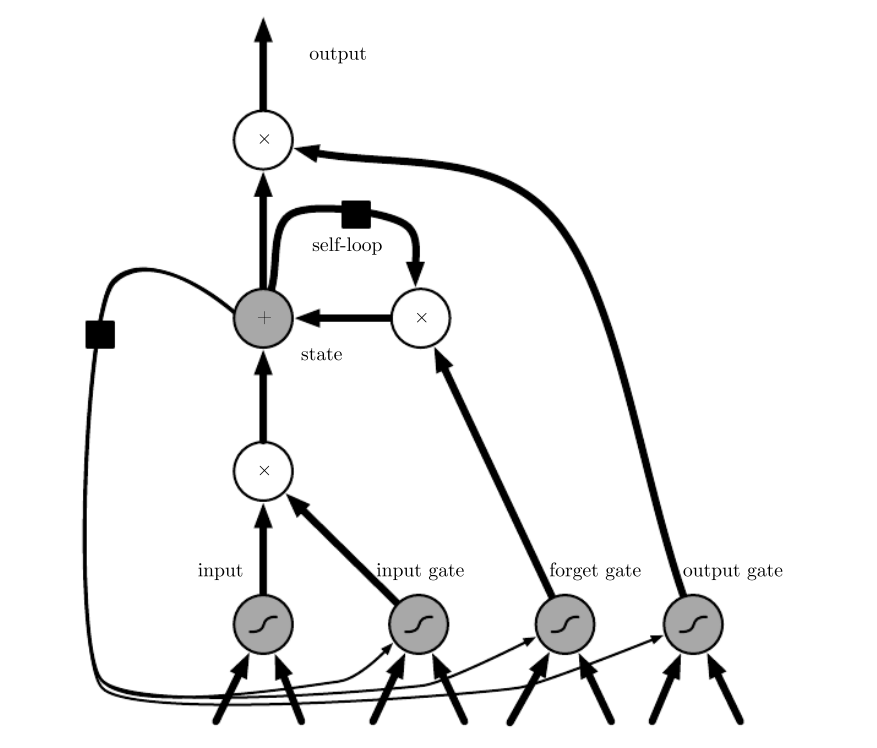
\includegraphics[scale=0.64]{lstm}\end{center}
\caption[lstm]{Štruktúra LSTM bunky}\label{fig:lstm}
\end{figure}

\begin{figure}[H]
\begin{center}
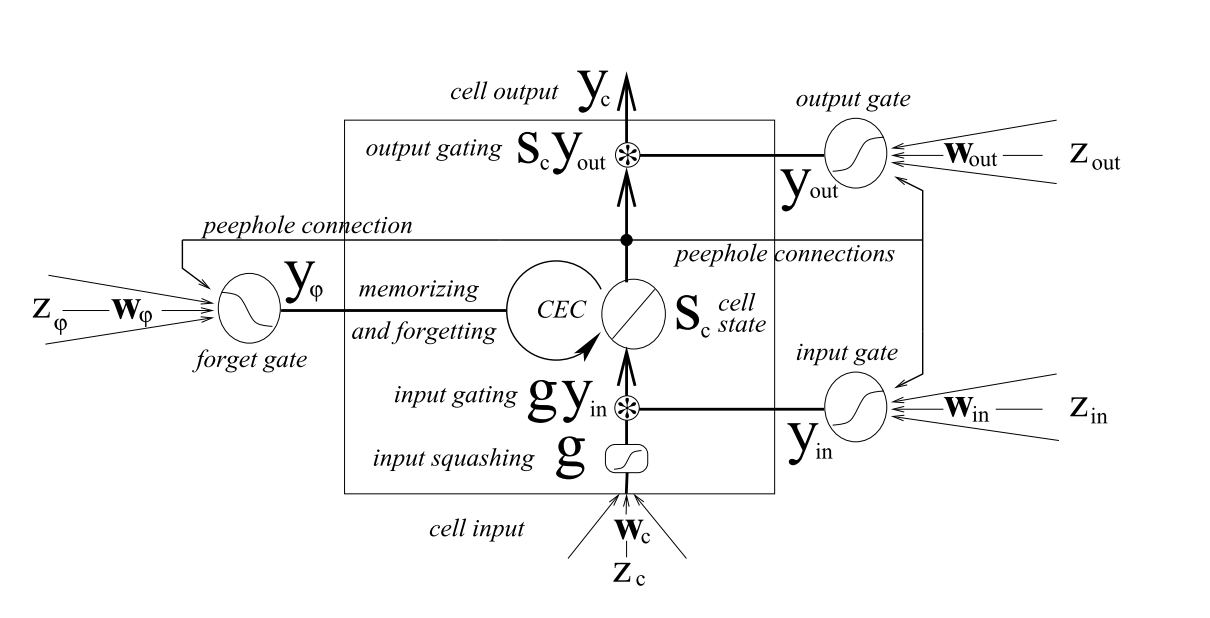
\includegraphics[scale=0.50]{peepholes}\end{center}
\caption[peepholes]{Schéma nazerania v LSTM bloku}\label{fig:peepholes}
\end{figure}

\section{Výskum v danej oblasti}
\label{analyza_vyskum_danej_oblasti}

V tejto časti sa zaoberáme štúdiou dostupných riešení pre problém úbytku zákazníkov. Zameriavame sa na metódy strojového učenia. Analýza poskytuje náhľad do konkrétneho biznis odvetvia, v ktorom bol skúmaný úbytok zákazníkov pre lepšie pochopenie stratégie, s ktorou bolo spracovanie dát a použité metódy optimalizované.

\subsection{Markovove reťazce, náhodné lesy}

Štúdia aplikuje štatistické modely, medzi nimi najúspešnejšie \textit{Markovove reťazce} a \textit{náhodné lesy} pri predikcii úbytku zákazníkov spoločnosti poskytujúcej káblovú televíziu. Skúmaná spoločnosť v minulosti rýchlo získala veľký podiel zákazníkov na trhu, o ktorý začala stabilne počas rokov prichádzať. Táto spoločnosť za použitia metód na predpovedanie úbytku zákazníkov dokázala takmer zdvojnásobiť svoje zisky zameriavaním sa na pozitívnu motiváciu najrizikovejších zákazníkov.
\newline
Spoločnosť ponúka stabilné ročné predplatné bez možnosti prerušenia zmluvy. Nahlasovanie plánovaného nepredlžovania zmluvy je povinné v poslednom mesiaci zmluvy, pričom neohlásenie automaticky predlžuje zmluvu na ďaľší rok. V štúdii boli sledovaní zákazníci, ktorí mali aktívnu zmluvu vo \textit{vzorkovacom dátume}(28. 2. 2002) a neboli vylúčení kvôli neplateniu predplatného. 
\newline
\subsubsection{Dataset}
\label{markov_dataset}
Dataset zákazníkov obsahuje nasledovné informácie o zákazníkoch:

\begin{my_itemize}
	\item{Zmluvné} - počet mesiacov trvania predplatného, mesiac ukončenia, typ produktu, špeciálne balíčky(šport, filmové, ...), spôsob platby
	\item{Socio-demografické} - vek, pohlavie, región, biznis
	\item{Finančné} - upomienky, typ upomienok, čas od poslednej upomienky
	\item{Historické} - počet obnov predplatného, získané zľavy 
\end{my_itemize}


Evidovaní zákazníci, ktorí opustili spoločnosť tvoria 15\% z datasetu. Pri využití metód bola vyhradená časť dát(60\%) pre kalibráciu a časť(40\%) pre testovanie úspešnosti. Stratifikácia bola aplikovaná kvôli udržaniu pomeru 15\% odchádzajúcich zákazníkov pre obe časti. %citovat  z clanku odkaz 

\subsubsection{Markovove reťazce}
\label{markov_markov}

Markovove reťazce sú pravdepodobnostná technika pre reprezentáciu korelácie medzi za sebou idúcimi pozorovaniami. Táto štúdia poukazuje na vplyv sekvencie v odoberanom type produktu na predpoveď, viď. tabuľku ~\ref{fig:producttable}. Kvôli tomuto javu boli využité Markovove reťazce. V minulosti boli úspešne aplikované na predikciu predaja finančných služieb, online predajov alebo na predpoveď úspešnosti softvéru.
%zdroj na obrazok aj minule aplikacie
\begin{figure}[H]
\begin{center}
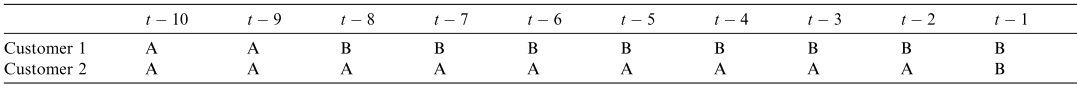
\includegraphics[scale=0.50]{producttable}\end{center}
\caption[producttable]{Sekvencia typu odoberanej služby dvoch zákazníkov}\label{fig:producttable}
\end{figure}

\subsubsection{Náhodné lesy}
\label{markov_lesy}

Kvôli svojej jednoduchosti použitia a interpretácie a schopnosti práce s ukazateľmi na rôznych úrovniach merania sa stali rozhodovacie stromy populárnou metódou predikcie. Ich nevýhody(ako napr. nedostatok robustnosti) úspešne rieši vytváranie veľkého počtu stromov so samostatným hlasovaním - lesov. Tento experiment využil náhodné lesy podľa štúdie L. Breimana. %Zdroj na Breimana

\subsubsection{Evaluácia}
\label{markov_evaluacia}

Štúdia pri evaluácii využíva počítanie zdvihu - pomeru zákazníkov predikovaných ako náchylných k prechodu a z nich zákazníkov, ktorí prešli inam, relatívne k percentu všetkých ušlých zákazníkov. Vysoký zdvih teda indikuje úspešný model. Pri 15,13\% úbytku zákazníkov teda perfektná predpoveď predstavuje $100/15,13 = 6,61$ zdvih. Na grafe~\ref{fig:lift} je možné vidieť úspešnosť jednotlivých metód pri vybratí daného percenta najohrozenejších zákazníkov. Vidno tu úspešnosť náhodných lesov aj takmer nulové zlepšenie logistickej regresie Markovovými reťazcami.

%zdroj na obrazok
\begin{figure}[H]
\begin{center}
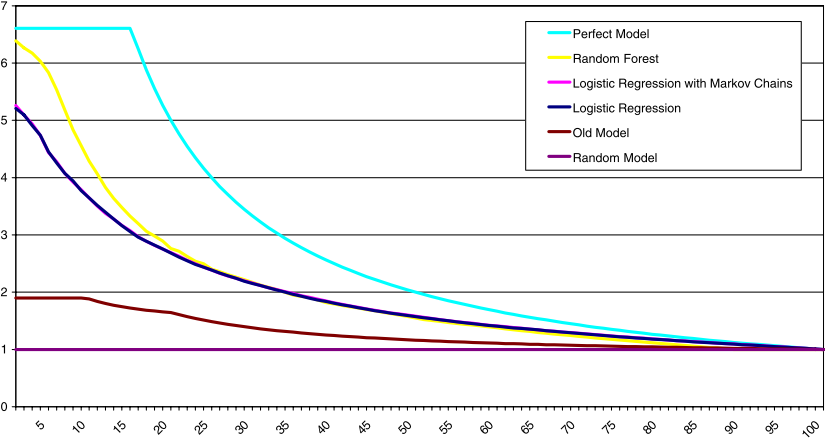
\includegraphics[scale=0.50]{lift}\end{center}
\caption[lift]{Výsledky použitých metód pre dané \% najohrozenejších zákazníkov}\label{fig:lift}
\end{figure}

\subsection{Neurónová sieť}
\label{metoda_neuronova_siet}

Neurónová sieť bola využitá pri štúdii zaoberajúcej sa predikciou úbytku zákazníkov u mobilného operátora. Zdanlivo jednoduchý model využívajúci učenie s učiteľom priniesol prekvapivo dobré výsledky pre verejne dostupný dataset.%odkaz na tuto studiu

\subsubsection{Dataset}
\label{nn_dataset}

Záznamy 20 rôznych premenných od 2427 zákazníkov obsahujú okrem samotnej informácie o úbytku nasledovné informácie:
\newline
štát, doba aktívnosti účtu, kód oblasti, telefónne číslo, medzinárodný plán (áno/nie), služba hlasového záznamu, počet hlasových záznamov, prevolané minúty (deň/večer/noc), počet hovorov(deň/večer/noc), (deň/večer/noc) platba, medzinárodné služby, počet volaní na zákaznícku linku.

\subsubsection{Neurónová sieť}
\label{metoda_nn}

Táto štúdia pracuje s klasickým modelom FNN pri predikcii. Ako prevencia problému preučenia funguje vyberanie náhodných záznamov do tréningového datasetu. Zbytok dát je využitých pre evaluáciu schopností siete predikovať úbytok.

Výsledná úspešnosť siete dosahuje 92,35\%. Architektúra tejto siete využíva jeden neurón pre každý vstup na prvej vrstve. Informácie o čísle a štáte neboli zahrnuté, lebo plnili iba identifikačnú funkciu. Po rozsiahlejších experimentoch so skrytými vrstvami sa ako najlepšie riešenie ukazuje využitie jedinej skrytej vrstvy s 3 neurónmi. Na výstupe neurónová sieť poskytuje informáciu o prechode(áno/nie) ale aj istotu, s ktorou tento výsledok určila. 
\newline
Na obr.~\ref{fig:importance} je tiež vidno, ako boli vyhodnotené jednotlivé vstupné parametre z hľadiska dôležitosti. Tá je určená na intervale $<0; 1>$, pričom však zriedka prekročí $0,35$. Ako sa ukázalo, najdôležitejším indikátorom prechodu zákazníka je počet volaní na zákaznícku podporu a množstvo medzinárodných služieb.

%zdroj na obrazok
\begin{figure}[H]
\begin{center}
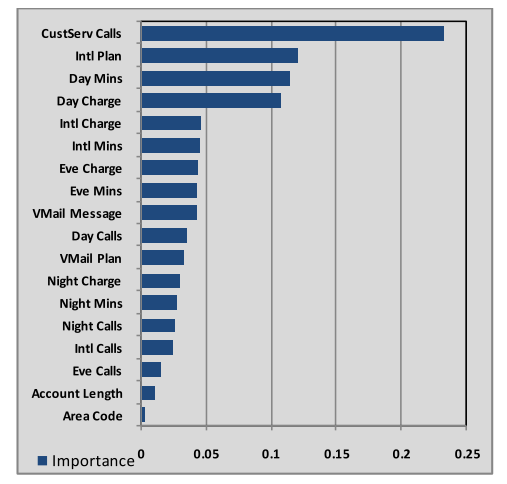
\includegraphics[scale=0.50]{importance}\end{center}
\caption[importance]{Vplyv parametrov na stratu zákazníka}\label{fig:importance}
\end{figure}

Tento model správne predikuje až 97\% ostávajúcich zákazníkov. Správne však určí iba 66\% strácaných zákazníkov. Evaluácia tohto výsledku je teda ťažko interpretovatelná hodnotou 92\%. 



\begin{comment}
\section{Časť}
\label{sec:Časť}
V tejto časti sa venujeme 
\begin{figure}[H]
\begin{center}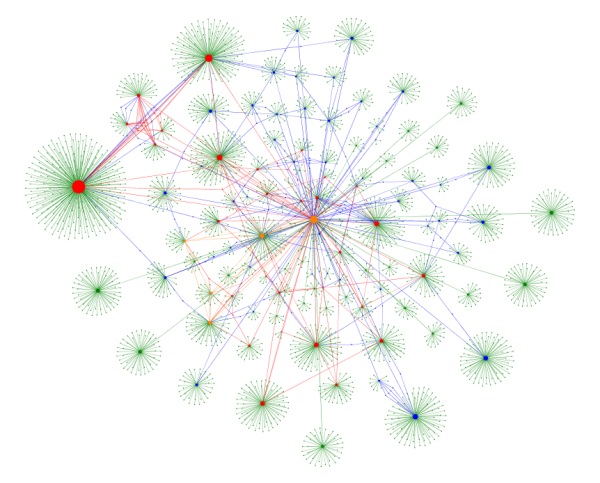
\includegraphics[scale=0.48]{figure}\end{center}
\caption[Name figure]{Name figure}\label{fig:figure}
\end{figure}

%\subsection{Enumeration}
\subsection{Číslovaný zoznam}
\begin{my_enumerate}
	\item {cieľ 1}
	\begin{my_enumerate}
		\item {cieľ 1.a}
		\item {cieľ 1.b}
	\end{my_enumerate}
	\item {cieľ 2}
	\item {cieľ 3}
\end{my_enumerate}

%\subsection{Citation}
\subsection{Citácia}
Lorem ipsum dolor sit amet, consectetuer adipiscing elit, sed diam nonummy nibh euismod tincidunt ut laoreet dolore magna aliquam erat volutpat~\cite{1}.

%\subsection{Labels \& References}
\subsection{Návestia \& Referencie}
Viď. sekcia~\ref{sec:Príklady}.\\
Viď. ukážka~\ref{fig:ukážka}.\\
Viď. číslovanie~\ref{lst:metrics_LOC}.\\
Viď. tabuľka~\ref{tab:tabuľka1}.

%\subsection{Examples}
\subsection{Príklady}
\label{sec:Príklady}

\begin{lstlisting}[ language=html, caption={Príklad 1}, label={lst:metrics_LOC},
	keywordstyle=\color{blue}\bfseries,
	ndkeywordstyle=\color{black}\bfseries,
	commentstyle=\color{red}\ttfamily,
	stringstyle=\color{green}\ttfamily,
	identifierstyle=\color{gray},
	backgroundcolor=\color{white}, 
	frame=single, 
	frameround=ffff,
	captionpos=b,
	basicstyle=\scriptsize
	]
<table class="metric_index">
	<tr>
		<th>Lines of code</th>
		<th>Value</th>
	</tr>
	<% if (filenum and modulenum) then %>
		<tr>
			<td class="name">Number of files</td>
			<td class="value"><%=filenum%></td>
		</tr>
		<tr>
			<td class="name">Number of modules</td>
			<td class="value"><%=modulenum%></td>
		</tr>
		<tr>
	<% end %>
	<tr>
		<td class="name">Lines Total</td>
		<td class="value"><%=LOC.lines%></td>
	</tr>
	<!--
							skryty zdrojovy kod
		podobne zobrazenie ostatnych metrik riadkov
	-->
</table>
\end{lstlisting}

\begin{lstlisting}[language=lua, caption={Názov}, label=metrics.pipe]
local parser  = require 'leg.parser'
local rules = require 'metrics.rules'
-- << skryty zdrojovy kod >> --
local capture_table = {}
grammar.pipe(LOC_capt.captures, AST_capt.captures)
grammar.pipe(block_capt.captures, LOC_capt.captures)
-- << viacero rovnakych volani s tabulkami captures inych modulov >> --
grammar.pipe(capture_table, cyclo_capt.captures)
local lua = lpeg.P(grammar.apply(parser.rules, rules.rules, capture_table))
local patt = lua / function(...) 
	return {...} 
end
local result = patt:match(code)[1]
\end{lstlisting}

\begin{lstlisting}[language=C++, tabsize=2, caption={Manager}]
int a;
\end{lstlisting}



\begin{table}[ht]
    \centering
    \begin{tabular}{ | l | l | }
    \hline
    Number of males & 51 \\ \hline
    Number of woman & 57 \\ \hline
    Gender not given & 27 \\ \hline
    Average age & 21,83 \\ \hline
    \end{tabular}
    \caption{Information about users}
    \label{tab:table1}
\end{table}

\end{comment}
